\chapter{Аналитический раздел}

В данном разделе производится формализация объектов сцены, анализ алгоритмов их визуализации, и выбираются наиболее подходящие для решения поставленных задач.

\section[Формализация объектов синтезируемой сцены]{Формализация объектов сцены}
\label{sec:obj_formalasation}

На визуализируемой сцене могут находиться следующие объекты:
\begin{enumerate}
	\item \textbf{Точечный источник света}
	
	Данный источник света испускает его равномерно во всех направлениях из фиксированной точки в трехмерном пространстве.
	Источник характеризуется:
	\begin{itemize}
		\item интенсивностью;
		\item позицией~\cite{Gambetta}.
	\end{itemize}
	
	\item \textbf{Рассеянный источник света}
	
	Привносит часть освещения в каждую точку сцены, независимо от ее расположения. 
	Источник характеризуется:
	\begin{itemize}
		\item интенсивностью~\cite{Gambetta}.
	\end{itemize}
	
	\item \textbf{Камера}
	
	В данном случае камера будет описана:
	\begin{itemize}
		\item матрицей проекции. Она определяет границы видимости в трехмерном пространстве;
		\item позицией.
	\end{itemize}
	
	\item \textbf{Трехмерные объекты}
		
	Трехмерные объекты будут описываться либо с помощью каркасной модели (во время морфинга), либо с помощью поверхностной модели (в статичном состоянии).
	Для этого задается:
	\begin{itemize}
		\item набор вершин;
		\item набор граней.
	\end{itemize}
\end{enumerate}


\section[Способ задания моделей]{Способ задания моделей}
\label{sec:method_set_models}

Для универсальности нашей программы выберем один из самых популярных форматов - .obj файлы. 
Файлы формата .obj (Wavefront OBJ) представляют собой текстовый формат, используемый для хранения трехмерных графических 
моделей. 
Они могут содержать следующую информацию:
\begin{itemize}
	\item \textbf{вершины} - координаты точек в трехмерном пространстве, которые определяют форму объекта;
	\item \textbf{нормали} - направления поверхности в каждой вершине, важные для расчета освещения;
	\item \textbf{текстурные координаты} - координаты, используемые для нанесения текстуры на поверхность модели;
	\item \textbf{грани} - определяют полигоны объекта, указывая индексы вершин, текстурных координат и нормалей, составляющих грани.
\end{itemize}

Поскольку мы будем использовать каркасные и поверхностные модели, из каждого файла нам нужно будет вычленять лишь вершины и грани. 
Таким образом, для определенного объекта будет составлен список его вершин, а также список граней, представляющих собой набор вершин.

\section[Анализ алгоритмов морфинга]{Анализ алгоритмов морфинга}
\label{sec:morph_algo}
\textbf{Морфинг} --- технология компьютерной графики, обеспечивающая плавный переход формы одного объекта в форму другого~\cite{morph_spheres}.

В последнее время наблюдается большой интерес к технологиям морфинга для создания плавных переходов между изображениями. 
Эти методы сочетают в себе 2D-интерполяцию формы и цвета для создания впечатляющих эффектов перехода.
Отчасти привлекательность морфинга заключается в том, что создаваемые изображения могут выглядеть поразительно реалистичными и визуально убедительными. 
Несмотря на то, что они вычисляются с помощью преобразований 2D-изображений, эффективные морфинги могут предполагать естественную трансформацию объектов в 3D-мире.

\subsection{Линейный морфинг}
Линейный морфинг (англ. Linear Morphing) является самым простым и распространенным подходом. 
Он основан на линейной интерполяции между начальными и конечными позициями каждой точки или вершины модели.
Путем изменения координат каждой точки по ходу времени, модель постепенно переходит из одной формы в другую~\cite{DMorph}.

Сам морфинг состоит из нескольких этапов: 
\begin{enumerate}
	\item Загрузка начальной и конечной модели морфинга, допускается несколько промежуточных состояний для плавности анимации.
	\item Переход между позициями вершин.
	\item Обновление текстурных координат.
	\item Расчет промежуточных геометрических состояний.
\end{enumerate}

\textbf{Переход между позициями вершин} --- для каждой вершины модели вычисляются ее промежуточные позиции между начальной и конечной точками.
Обычно это достигается путем линейной интерполяции координат вершин по временному параметру, который определяет текущий прогресс между началом и концом морфинга.

\textbf{Обновление текстурных координат} --- аналогично с расчетом промежуточных позиций вершин необходимо с помощью интерполяции расчитать текстурные координаты.

\textbf{Расчет промежуточных геометрических состояний} --- на основе расчитанных ранее координат возможно получить промежуточные геометрические состояния модели~\cite{DMorph}.

\begin{figure}[h]
	\centering
	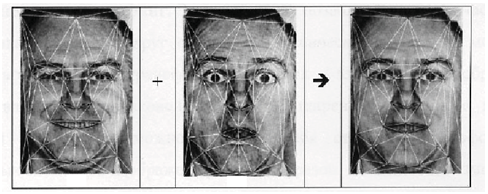
\includegraphics{images/morhing_faces.png}
	\caption{Пример линейного морфинга человеческого лица}
	\label{fig:morhing_faces}
\end{figure}

\newpage

\textbf{Плюсы:}
\begin{enumerate}
	\item Вычислительные затраты меньше, чем у других алгоритмов~\cite{morphing_methods}.
\end{enumerate}

\textbf{Минусы:}
\begin{enumerate}
	\item Ограниченные возможности для создания сложных форм и детализации.
	\item Ограниченный контроль над динамическими атрибутами, такими как цвета или нормали.
	\item Не всегда способен обеспечить реалистичный морфинг для моделей с большим количеством вершин или сложной геометрией~\cite{morphing_methods}.
\end{enumerate}


\subsection{Весовая деформация}
Идея данного метода аналогична методу, описанному в~\ref{sec:morph_algo}, однако в данном случае каждая из вершин имеет собственный вес.
Изначально каждая вершина присваивается какой-либо части тела объекта (кости). 
Каждая вершина модели привязывается к костям с помощью весов. 
Вес определяет, насколько каждая кость влияет на вершину. 
Чаще всего веса представлены числами от 0 до 1, где 0 означает полное отсутствие влияния, а 1 --- полное влияние соответствующей кости. 
Весовые значения для каждой вершины нормализуются, так чтобы сумма весов для каждой вершины была равна 1. 
Это позволяет равномерно распределить влияние костей и избежать нежелательных артефактов. 
В процессе анимации, для каждого кадра, путем комбинирования позиций и ориентаций костей с их соответствующими весами, определяются новые позиции вершин.
Это достигается путем линейной интерполяции или других методов комбинирования весовых значений и позиций костей~\cite{weight_morphing}.

\begin{figure}[h]
	\centering
	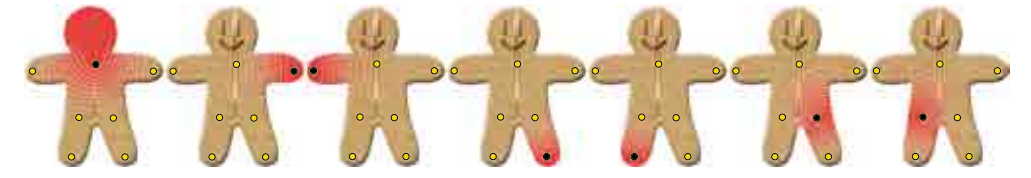
\includegraphics[scale=0.8]{images/stickman_weights.png}
	\caption{Иллюстрация веса вершины в зависимости от ее положения}
	\label{fig:stickman_weights}
\end{figure}
На картинке~\ref{fig:stickman_weights} с помощью интенсивности красного цвета показывается значение веса вершины в зависимости от ее положения.

\begin{figure}[H]
	\centering
	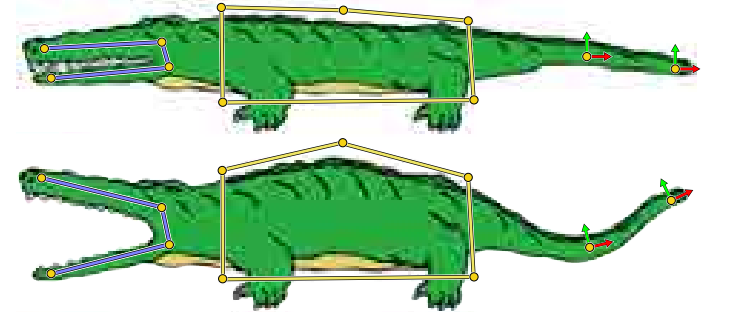
\includegraphics{images/weight_points_chosen.png}
	\caption{Пример выбора вершин на скелете}
	\label{fig:weight_points_chosen}
\end{figure}

\textbf{Плюсы:}
\begin{enumerate}
	\item Гибкость в управлении деформацией и анимацией модели.
	\item Возможность создания более сложных форм и эффектов деформации.
	\item Мощный инструмент для контроля за определенными частями модели в процессе морфинга~\cite{morphing_methods}.
\end{enumerate}

\textbf{Минусы:}
\begin{enumerate}
	\item Дополнительная сложность в настройке и установке весовых значений для каждой вершины.
	\item Проблемы с поддержкой ненатуральных или сложных деформаций.
	\item Возможность создания артефактов, таких как рывки или изломы~\cite{morphing_methods}.
\end{enumerate}

\subsection{Морфинг на основе ключевых точек}
При использовании данного метода морфинга выделяются несколько промежуточных этапов (точек) перехода одного объекта в другой. После чего, для каждого промежуточного этапа каждой вершине из предыдущего этапа ставится в соответствие вершина из последующего. 
Далее, для перехода из одного этапа в другой используется интерполяция.

\begin{figure}[H]
	\centering
	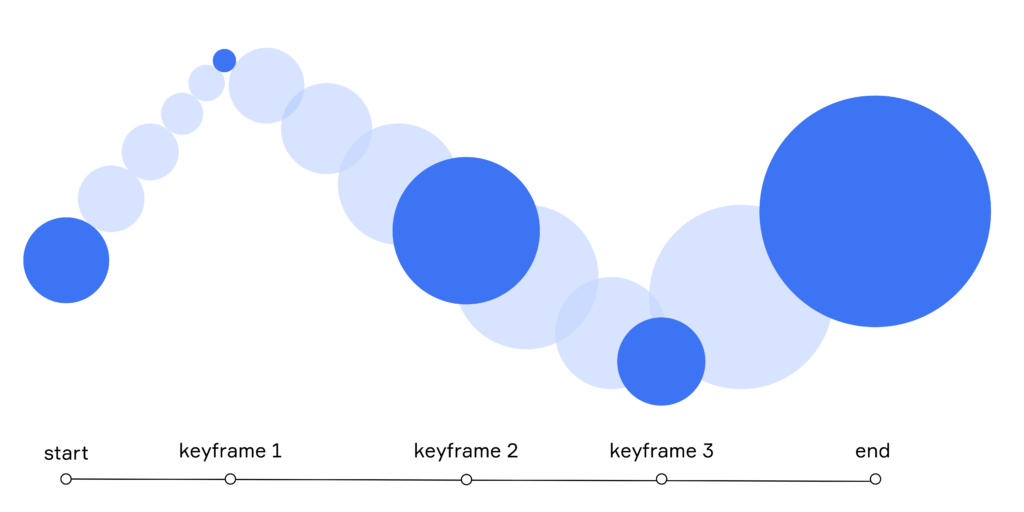
\includegraphics[scale=0.4]{images/key_frames.png}
	\caption{Пример выделения ключевых точек}
	\label{fig:key_frames}
\end{figure}


\textbf{Плюсы:}
\begin{enumerate}
	\item Хорошая контролируемость и предсказуемость в анимации и морфинге моделей.
	\item Возможность создания точных и выразительных анимаций с помощью набора ключевых точек.
	\item Гибкость в управлении настройками и характеристиками каждой ключевой точки~\cite{morphing_methods}.
\end{enumerate}

\textbf{Минусы:}
\begin{enumerate}
	\item Необходимость тщательного планирования и размещения ключевых точек для достижения предполагаемого эффекта.
	\item Ограничение в контроле над промежуточными состояниями между ключевыми точками.
	\item Увеличение объема данных при использовании большого числа ключевых точек~\cite{morphing_methods}.
\end{enumerate}

\textbf{Вывод:}

Проанализировав алгоритмы морфинга можно прийти к выводу, что наилучшим методом для решения поставленной задачи является линейный морфинг (англ. Linear morphing), так как он является наиболее быстродействующим из представленных алгоритмов, что играет значимую роль при большом количестве примитивов.


\section{Анализ алгоритмов закраски}
\label{sec:draw_algo_analysis}
Для сглаживания и добавления реализма изображениям можно использовать алгоритмы закраски.
В данном случае будут рассмотрены 3 основных алгоритма закраски:
\begin{enumerate}
	\item Простая закраска.
	\item Закраска методом Гуро.
	\item Закраска методом Фонга~\cite{draw_methods}.
\end{enumerate}

\subsection{Простая закраска}
В случае использования простой закраски считается, что и источник света и наблюдатель находятся в бесконечности,
так что диффузная составляющая одинакова (она зависит от угла падения), вектор наблюдения также будет для всех точек одинаковым, то есть зеркальная составляющая также не будет изменяться. 
Таким образом данный алгоритм является быстрым, однако в случае, если закрашиваемая грань является результатом аппроксимации тела, будет заметен резкий переход между интенсивностями~\cite{Rodgers}.

\textbf{Плюсы:}
\begin{enumerate}
	\item Простая реализация.
	\item Время реализации меньше, чем у других алгоритмов~\cite{Rodgers}.
\end{enumerate}

\textbf{Минусы:}
\begin{enumerate}
	\item Очень низкая реалистичность~\cite{Rodgers}.
\end{enumerate}


\subsection{Закраска методом Гуро}
В случае использования метода Гуро можно получить сглаженное изображение, для этого сначала определяется интенсивность вершин многоугольника, а затем с помощью билинейной интерполяции вычисляется интенсивность каждого пикселя на сканирующей строке.

\begin{figure}[H]
	\centering
	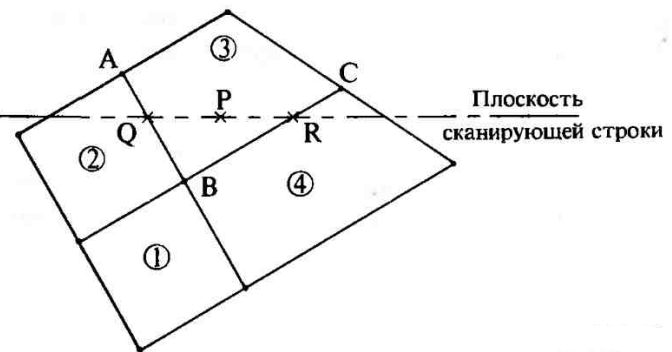
\includegraphics{images/guro.png}
	\caption{Пример полигональной поверхности}
	\label{fig:guro_polygon}
\end{figure} 

Например, рассмотрим участок полигональной поверхности на рисунке~\ref{fig:guro_polygon}.
Значение интенсивности в точке P
определяется линейной интерполяции значений интенсивностей в точках Q и R.
Для получения интенсивности в точке Q можно провести линейную интерполяцию интенсивности в вершинах A и B по формуле
\begin{equation} 
	I_Q = uI_A+(1-u)*I_B  \quad 0 \leq u \leq 1, t = \frac{AQ}{AB}.
	\label{eq:guro_inter_1}
\end{equation}

Таким же образом рассчитывается интенсивность в точке B, после чего интерполяция используется еще раз, для поиска значения интенсивности в точке P~\cite{Rodgers}.
\begin{equation} 
	I_P = tI_Q+(1-t)*I_R  \quad 0 \leq t \leq 1, t = \frac{QP}{QR}.
	\label{eq:guro_inter_2}
\end{equation}

\newpage

\textbf{Плюсы:}
\begin{enumerate}
	\item Получение сглаженного изображения.
	\item Трудозатраты меньше, чем у любого другого алгоритма, кроме алгоритма простой закраски~\cite{Rodgers}.
\end{enumerate}

\textbf{Минусы:}
\begin{enumerate}
	\item Появление полос Маха - оптической иллюзии. 
	Она преувеличивает контраст между краями слегка отличающихся оттенков, в местах, где они соприкасаются друг с другом.
	\item Не учитывает кривизны поверхности (случай, если нормали поверхностей одинаково ориентированы)~\cite{Rodgers}.
\end{enumerate}


\subsection{Закраска методом Фонга}
Закраска Фонга требует больших вычислительных затрат, однако она решает множество проблем метода Гуро.
В данном методе вместо интерполяции интенсивностей света, производится интерполяция вектора нормали.
Таким образом учитывается кривизна поверхности.
В случае рисунка~\ref{fig:guro_polygon}, нормали в соответствующих точках рассчитывалась бы формулами~\ref{eq:phong_shading}~\cite{Rodgers}.
\begin{equation}
	\label{eq:phong_shading}
	\begin{aligned}
		n_Q = un_A + (1-u)n_B  \quad 0 \leq u \leq 1 \\
		n_R = wn_B + (1-w)n_C  \quad 0 \leq w \leq 1 \\
		n_P = tn_Q + (1-t)n_R  \quad 0 \leq t \leq 1.
	\end{aligned}
\end{equation}
где
\begin{equation}
	\begin{aligned}
		u = \frac{AQ}{AB} \\\\
		w = \frac{BR}{BC} \\\\
		t = \frac{QP}{QR} 
	\end{aligned}
\end{equation}

\newpage

\textbf{Плюсы:}
\begin{enumerate}
	\item Получение сглаженного изображения.
	\item Учет кривизны поверхностей.
	\item Улучшенная реалистичность зеркальных бликов (по сравнению с методом Гуро)~\cite{Rodgers}.
\end{enumerate}

\textbf{Минусы:}
\begin{enumerate} 
	\item Трудозатратность алгоритма больше, чем у других алгоритмов~\cite{Rodgers}.
\end{enumerate}


\textbf{Вывод:}

На рисунке~\ref{fig:shading_compare} представлены различные методы закраски. 
Заметим, что наиболее подходящей закраской для поставленной задачи является закраска Гуро, так как мы будем использовать модели с большим количеством примитивов и нам будет важна производительность. При этом вычислительных способностей достаточно, чтобы не использовать простую закраску.

\begin{figure}[H]
	\centering
	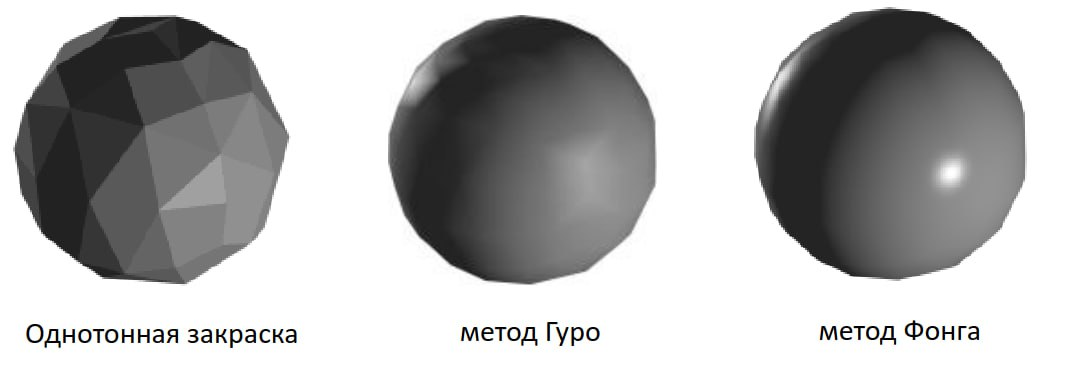
\includegraphics[scale=0.6]{images/shading_compare.jpg}
	\caption{Сравнение методов закраски}
	\label{fig:shading_compare}
\end{figure}


\section{Анализ алгоритмов удаления невидимых линий и поверхностей}

В рамках данной работы для визуализации процесса морфинга необходимо отсекать невидимые поверхности, для решения поставленной
существует множество алгоритмов.

\subsection{Алгоритм Робертса}
Преимуществом этого алгоритма является его эффективное использование мощных и точных математических методов. 
На первом этапе происходит удаление ребер или граней, которые находятся за самим объектом, а затем рассматриваются грани, закрытые другими объектами на сцене. 
Если объекты пересекаются друг с другом, удаляются невидимые линии пересечения. 
Однако недостатком алгоритма является то, что вычислительная сложность растет квадратично с увеличением числа объектов,
что может привести к замедлению работы алгоритма в случае большого числа объектов на сцене.
Приведенный недостаток является критически важным для поставленно задачи, однако возможна модификация с использованием 
сортировки по оси Z, что улучшит производительность алгоритма~\cite{Rodgers}.

\subsection{Алгоритм Z-буфера}
Данный алгоритм позволяет не только удалять невидимые линии и поверхности, но и визуализировать их пересечение.
При работе данного алгоритма происходит поиск наиближайшего объекта к каждому пикселю экрана.
Сцена может быть любой сложности, а так как размер изображения ограничен размером экрана, сложность алгоритма зависит линейно от количества поверхностей. 

У этого алгоритма есть и существенные недостатки. 
Он требует больший объем памяти для своей реализации, так как необходимо хранить буфер кадра и Z-буфер.
Кроме того, его сложно использовать для реализации эффектов, таких как прозрачность и освещение, ввиду отсутствия 
наблюдения за лучами света~\cite{Rodgers}.

\begin{figure}[H]
	\centering
	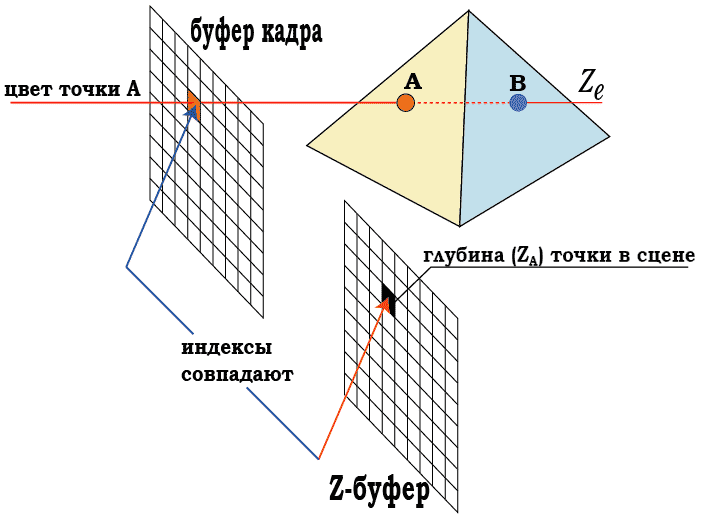
\includegraphics[scale=0.67]{images/z_buf.png}
	\caption{Пример работы алгоритма, использующего Z-буфер}
	\label{fig:zbuf}
\end{figure}

\subsection{Обратная трассировка лучей}
В данном алгоритме предполагается, что точка зрения находится в бесконечности на положительной полуоси Z, что делает все световые лучи параллельными этой оси. 
Алгоритм отслеживает траекторию каждого луча и определяет, с какими объектами сцены, если они существуют, он пересекается.
В случае если пересечение существует, то из данного луча образуются преломленный и отраженный.

Благодаря этому алгоритму можно достичь эффектов, таких как отражение и преломление, что делает изображение более реалистичным. 
Каждый пиксель изображения вычисляется независимо от других, что обеспечивает высокую параллельность расчетов.

Однако алгоритм обратной трассировки лучей имеет и недостатки.
Данный алгоритм очень ресурсоемок, так как каждый луч порождает несколько отраженных и преломленных лучей, которые также необходимо хранить и обрабатывать.
Также для поиска пересечения одного луча необходимо проанализировать все имеющиеся на сцене примитивы, что значительно влияет на вычислительную сложность алгоритма~\cite{Rodgers}.

\begin{figure}[H]
	\centering
	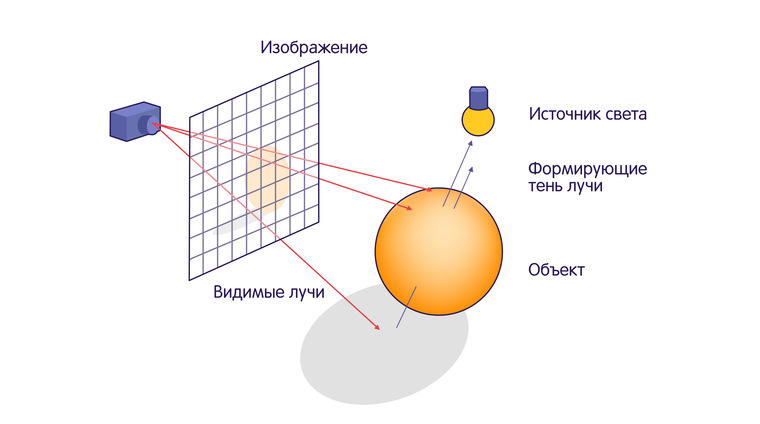
\includegraphics[scale=3]{images/ray_traycing.jpeg}
	\caption{Пример работы алгоритма обратной трассировки лучей}
	\label{fig:ray_traycing}
\end{figure}

\textbf{Вывод}

Проанализировав алгоритмы удаления невидимых линий и поверхностей, заметим, что для поставленной задачи больше всего подходит алгоритм Z-буфера, так как он может работать со сценами любой сложности и не требует больших вычислительных мощностей для сцен с множеством объектов, что необходимо при реализации морфинга.


\section*{Выводы из аналитического раздела}

В данном разделе были проанализированы алгоритмы морфинга, удаления невидимых линий, а также методы закраски.
Таким образом были выбраны следующие алгоритмы.
\begin{enumerate}
	\item \textbf{Алгоритм морфинга} - линейный морфинг.
	\item \textbf{Метод закраски} - закраска Гуро.
	\item \textbf{Алгоритм удаления невидимых линий} - алгоритм Z-буфера.
\end{enumerate}

Входными данными для полученной системы будут являться:
\begin{itemize}
	\item вершины и ребра модели;
	\item локальные координаты модели;
	\item угол поворота модели по каждой оси;
	\item текущий масштаб модели;
	\item положение камеры;
	\item положение источника света.
\end{itemize}